% !Mode\dots ``TeX:UTF-8''
% !TEX root = ../bare_jrnl.tex
\section{Introduction}
\label{sec:intro}


%Before introducing the Boolean control networks, we introduce the Boolean networks at first. 
In 1960s, Nobel Prize laureates Jacob and Monod found that ``Any cell contains a number of `regulatory' genes that act as switches and can turn one another on and off. If genes can turn one another on and off, then you can have genetic circuits.''\cite{Jacob1961Genetic} Inspired by these Boolean-type actions in genetic circuits, Boolean networks (\BNs) were firstly proposed by Kauffman \cite{Kauffman1968Metabolic} for modeling nonlinear and complex biological systems. 

{\BNs} are a type of discrete systems which are based on a directed graph. In a Boolean network, each node has only two states ``0" and ``1", and
the node's state can change in different time steps.  For a node $n_i$, we use $n_i(t)$ to denote the state of $n_i$ at time step $t$.
%
The value of $n_i(t+1)$ is decided by a logical function of  set of  values  $\{n_j(t),\ldots,n_p(t)\}$ if  there are directed edges from $n_j,\ldots,n_p$ to $n_i$.  % We call nodes as $n_j,\ldots,n_p$ are the neighboring nodes of $n_i$ %\ly{In \BNs,   $n_i(t+1)$ is obtained through logical operations on the  neighboring nodes' value at time $t$.} 
 The logical operators used in  logical function include: AND, OR, NO, XOR. %\ly{, and so on, "delete"}. 
Some general descriptions of the \BNs\ and their applications to biological systems can be found in \cite{Kauffman1968Metabolic}.
There are many natural and artificial systems works \cite{Akutsu2000Inferring, Shmulevich2002From, Faur2006Dynamical,Green2007The,Lou2010Multi} related to \BNs.
 

\BNs\ can be naturally extended to Boolean control networks (\BCNs) when external regulation or perturbation is considered \cite{Ideker2001A}. There are three kinds of nodes in \BCNs, \ly{including input-nodes ($\mathfrak{i}$), state-nodes ($\mathfrak{s}$) and output-nodes ($\mathfrak{o}$).} In \BCNs, we can only control input-nodes and observe output-nodes. 
%While, there is no edge with target in input-nodes, and no edge starts from the output-nodes. 
The value of each state-node $\mathfrak{s}_i(t+1)$ is decided by a logical function of  $\{\mathfrak{s}_j(t),\ldots,\mathfrak{s}_p(t),\mathfrak{i}_x(t),\ldots,\mathfrak{i}_y(t)\}$  %if there are directed edges from $\mathfrak{s}_j,\ldots,\mathfrak{s}_p,\mathfrak{i}_x,\ldots,\mathfrak{i}_y$ to $\mathfrak{s}_i$ 
while the value of each output-node $\mathfrak{o}_i(t)$ is decided by a logical function of   $\{\mathfrak{s}_j(t),\ldots,\mathfrak{s}_p(t)\}$. 
%if  there are directed edges from $\mathfrak{s}_j,\ldots,\mathfrak{s}_p$ to $\mathfrak{o}_i$.
%However,  the value of node $n_i$ can be reflected by the value of  node $n_j$ if there exists a 
%path from $n_j$ to $n_i$. Therefore,  the value of node $n_i(k)$  is decided by initial state of state nodes and the value of input-nodes  at time step $0,\cdots, k$.

%\begin{comment}
%{\textcolor{blue}{ Too many words, delete?}}\ly{  The value of each state-node \State$_i(t)$ can be reflected by the value of an output-node \Output$_i(t)$ if there exists a directed edge from \State$_i$ to \Output$_i$. And the value of each state node \State$_i(t+1)$ at the next time step is affected by the value of a state-node \State$_j(t)$ (or an input-node \Input$_i(t)$) if there is a directed edge from \State$_j$ (or \Input$_i$) to \State$_j$, where \State$_i$ and \State$_j$ can be the same node. Therefore, there are also a series of logical operations (updating rules) to obtain the new values of the state nodes and output nodes of \BCNs. } 
%\end{comment}

\BCNs\ can be used to solve various real-life problems, for instance, %first \BCNs\ have been used to do 
structural and functional analysis of signalling and regulatory networks \cite{Kaufman1999A, Klamt2006A}, 
%. Second \BCNs\ have been used for 
abduction based drug target discovery \cite{Biane2017Abduction}, %. Furthermore, \BCNs\ also have been used for 
and pursuing evasion problems in polygonal environments \cite{Thunberg2011A}. 




%By this method, we can study the properties of the 

 %\begin{figure}[thpb]
    %  \centering
      %\framebox{\parbox{3in}{
	%	\centerline{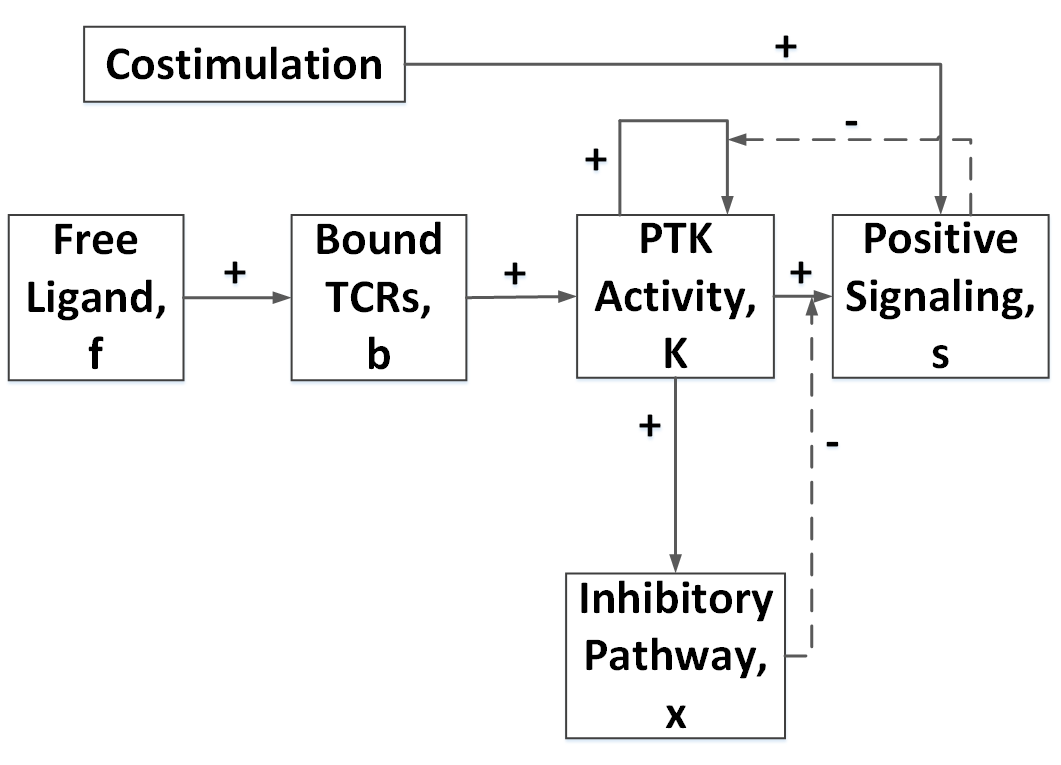
\includegraphics[scale=0.277]{figures/Fig6.png}}
	%}}
      
     % \caption{Schematic interaction diagram. f = free ligand; b = TCRs
%bound to ligand; k = receptor-associated PTK activity; x = tyrosine
%kinase-dependent inhibitory pathway; s = metabolic and mitogenic
%response. Positive and negative interactions are indicated by a plus and
%minus sign, respectively.}
  %    \label{fig:6}
  %\end{figure}

%As the wide application of \BCNs, there are a lot of research work about 
We are mainly interested in the control-theoretic problems of \BCNs. The work \cite{Akutsu2007Control} proves that the problem of determining the controllability of \BCNs\ is {\bf NP}-hard in the number of nodes. In addition, it points out that ``One of the major goals of systems biology is to develop a control theory for complex biological systems.'' Since then, the study on control-theoretic problems in the areas of \BNs\ and \BCNs\ has drawn great attention \cite{cheng2009controllability, Zhao2010Input, Cheng2011Identification, Cheng2011Analysis,Fornasini2013Observability}. What is more, the controllability and observability are the basic control-theoretic problems of \BCNs. % Among these studies, \emph{semi-tensor product} (\STP) is one of useful tools to deal with  both \BNs\ and \BCNs\  related problems \cite{cheng2009controllability}.  We will refer to \STP\ in the {\em Section \ref{sec:pre}}. Moreover,  the concept of \BCN\'s observability was proposed firstly in \cite{cheng2009controllability}. 

%\ly{Observability is one of \BCNs' control-theoretic problems.} 
%In this paper we research the observability of the \BCNs. 

The concept of observability was proposed firstly in \cite{cheng2009controllability}. To date, there are four types of observability have been proposed. And they are mainly about how to get  information of the initial value of the state-nodes of the \BCNs\ by the value of their input-nodes and output-nodes. 
%\ly{
%Because the value of state-nodes can be reflected by the value of output-nodes. And, the value of state-nodes at the next time step is affected by the value of state-nodes and input-nodes. Such that
% In \BCNs, we can control the new value of the state-nodes by the value of input-nodes. And we can  predict the last value of state-nodes by the value of output-nodes.   Therefore, with the updating rules of \BCNs\ we can infer  the initial value of state-nodes of \BCNs\ by the value of input-nodes and output-nodes.} % Then based on actual application needs, different types of observability are defined to get different kinds of information about the initial value of state-nodes%Therefore, we can get some information about the initial state $s_0$ by the output of the \BCN.
%If there are multipal type of initial state $s_0$ of a \BCN\ with the same output $o_0$, then we can not determine the initial state by the initial output. 
% Then, we can use the input to control the state of \BCNs, and then get more information about the new state by the new output we observed. So that, we can get more information about the initial state of \BCN\ by controlling the input.

\tl{do you use  gothic to denote vectors? this paragraph is repeating} 
For convenience, we use the vectors input $\mathfrak{i}(t)$, state $\mathfrak{s}(t)$, and output $\mathfrak{o}(t)$ to represent the value of all input-nodes, all state-nodes and all output-nodes, respectively. Then we have $\mathfrak{s}(t+1)$ is decided by $\mathfrak{i}(t)$ and $\mathfrak{s}(t)$, and $\mathfrak{o}(t)$ is decided by $\mathfrak{o}(t)$ as shown in Fig.\ref{fig:10}.


 \begin{figure}[thpb]
      \centering
      \framebox{\parbox{3in}{
		\centerline{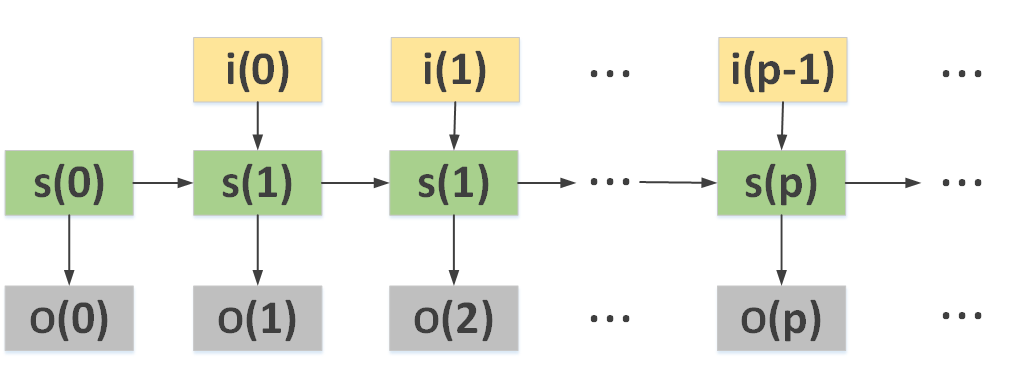
\includegraphics[scale=0.28]{figures/Fig10.png}}
	}}
      
      \caption{The relationship of input, state and output.}
      \label{fig:10}
  \end{figure}
   The sequences $\mathfrak{i}(0)$$\mathfrak{i}(1)\ldots$
$\mathfrak{i}(k-1)$,  $\mathfrak{s}(0) $$\mathfrak{s}(1)\ldots$$\mathfrak{s}(k)$, and $\mathfrak{o}(0)$$\mathfrak{o}(1)\ldots$$\mathfrak{o}(k)$ 
 consists of several inputs, states and outputs  in sequential time steps,  respectively. 
 Such that, for a initial state $\mathfrak{s}(0)$ and a $\mathfrak{i}(0)$$\mathfrak{i}(1)\ldots$$\mathfrak{i}(k-1)$ of a \BCN, we have their corresponding 
$\mathfrak{s}(0)$$\mathfrak{s}(1)\ldots $$\mathfrak{s}(k)$ and $\mathfrak{o}(0) $$\mathfrak{o}(1)\ldots$ $\mathfrak{o}(k)$.  
Then for a given  \BCN\  $\BB$,  $\mathfrak{o}(0)$$\mathfrak{o}(1)\ldots$ $\mathfrak{o}(k)$ is decide by
$\mathfrak{s}(0)$ and sequence $\mathfrak{i}(0)$$\mathfrak{i}(1)\ldots$$\mathfrak{i}(k-1)$. 
 
 Thus one of the main problems of observability can been described as: 
 \tl{this is not a well defined question, because you do not know whether such an input exists or not ;-), and $k$ is unspecified. }
\begin{problem}
\label{pro:1}
For a given  \BCN, how to get $\mathfrak{i}(0)$$\mathfrak{i}(1)\ldots$$\mathfrak{i}(k-1)$, so that we can determine the initial state $\mathfrak{s}(0)$?
\end{problem}
%In this paper, we are focus on this problem.

As  mentioned before, there are four types of observability. 
\tl{???}The $\mathfrak{s}^{i}(t)$ and $\mathfrak{s}^{j}(t)$ represent different valuations of state-nodes, so do input-nodes and output-nodes. Then four existing observability of \BCNs\ are as follows. 
%A output can be seen as a vector of the values of all output-nodes of the \BCN\ in a time step as well. Therefore a output sequence also consists of several outputs in sequential time steps. 
%Moreover,  \cite{cheng2009controllability} gives equivalent conditions for controllability of \BCNs\ and observability of controllable \BCNs. 

\ly{I suggest that using formulas to represent for existing observabilities.}

\tl{from these descriptions, it is hard to tell the differences of the definitions}

\begin{enumerate}
	\item The first type of observability was proposed in 2009 \cite{cheng2009controllability}, and it states that for every $\mathfrak{s}^{i}(0)$ there is an $\mathfrak{i}(0)$$\mathfrak{i}(1)\ldots$$\mathfrak{i}(k-1)$ that can be used to distinguish it from other types of initial states. Because for this $\mathfrak{i}(0)$$\mathfrak{i}(1)\ldots$$\mathfrak{i}(k-1)$, for every $\mathfrak{s}^{j}(0)\ne$$\mathfrak{s}^{i}(0)$, the corresponding $\mathfrak{o}^{i}(0)$$\mathfrak{o}^{i}(1)\ldots$$\mathfrak{o}^{i}(k)$ of $\mathfrak{s}^{i}(0)$ is different from the corresponding $\mathfrak{o}^{j}(0)$$\mathfrak{o}^{j}(1)\ldots$$\mathfrak{o}^{j}(k)$ of $\mathfrak{s}^{j}(0)$. %Therefore, we can distinguish the \State$^{i}(0)$  by this input sequence, and then we can determine whether \State$(0)=$\State$^{i}(0)$.
	%------------------------------
	\item 
	The second observability was proposed in 2010 \cite{Zhao2010Input}, and it is determined in \cite{Li2015Controllability}. It stands that for every two distinct $\mathfrak{s}^{i}(0)$ and $\mathfrak{s}^{j}(0)$, there exists an $\mathfrak{i}(0)$$\mathfrak{i}(1)\ldots$$\mathfrak{i}(k-1)$ that can be used to distinguish them. Because for this $\mathfrak{i}(0)$$\mathfrak{i}(1)\ldots$$\mathfrak{i}(k-1)$, the corresponding $\mathfrak{o}^{i}(0)$$\mathfrak{o}^{i}(1)\ldots$$\mathfrak{o}^{i}(k)$ of $\mathfrak{s}^{i}(0)$ and the corresponding $\mathfrak{o}^{j}(0)$$\mathfrak{o}^{j}(1)\ldots$$\mathfrak{o}^{j}(k)$ of $\mathfrak{s}^{j}(0)$ are different. %Therefore, we can distinguish \State$^{i}(0)$ and \State$^{j}(0)$ by this input sequence, and then we can determine whether the initial state \State$(0)$ is \State$^{i}(0)$ or \State$^{j}(0)$.	
	\item The third observability proposed in 2011 \cite{Cheng2011Identification}, and it states that there is an $\mathfrak{i}(0)$$\mathfrak{i}(1)\ldots$$\mathfrak{i}(k-1)$ that determines $\mathfrak{s}(0)$. Because for this $\mathfrak{i}(0)$$\mathfrak{i}(1)\ldots$$\mathfrak{i}(k-1)$, for every two distinct $\mathfrak{s}^{i}(0)$ and $\mathfrak{s}^{j}(0)$, the corresponding $\mathfrak{o}^{i}(0)$$\mathfrak{o}^{i}(1)\ldots$$\mathfrak{o}^{i}(k)$ of $\mathfrak{s}^{i}(0)$ is different from the corresponding $\mathfrak{o}^{j}(0)$$\mathfrak{o}^{j}(1)\ldots$$\mathfrak{o}^{j}(k)$ of $\mathfrak{s}^{j}(0)$.
	
	\item  The fourth observability proposed in 2013 \cite{Fornasini2013Observability} is essentially the observability of linear control systems, i.e., that every sufficient long $\mathfrak{i}^{x}(0)$$\mathfrak{i}^{x}(1)\ldots$ $\mathfrak{i}^{x}(k-1)$ can determine $\mathfrak{s}(0)$. Because for this $\mathfrak{i}^{x}(0)$$\mathfrak{i}^{x}(1)\ldots$ $\mathfrak{i}^{x}(k-1)$, for every two distinct $\mathfrak{s}^{i}(0)$ and $\mathfrak{s}^{j}(0)$, the corresponding $\mathfrak{o}^{i}(0)$$\mathfrak{o}^{i}(1)\ldots$$\mathfrak{o}^{i}(k)$ of $\mathfrak{s}^{i}(0)$ is different from the corresponding $\mathfrak{o}^{j}(0)$$\mathfrak{o}^{j}(1)\ldots$$\mathfrak{o}^{j}(k)$ of $\mathfrak{s}^{j}(0)$.%Therefore, we can determine the initial state of the \BCN\ by every sufficient long input sequence for every initial state \State$(0)$.
\end{enumerate}
 The formal definition will be presented completely in {\em Section \ref{sec:pre}}.
%\tl{can you state the four types observability clearly and formally here?}

%\rev{****input s equence***}

 % in the following pages. What's more, there is an approach to study large-scale \BCNs\ via network aggregations \cite{Zhang2017Observability}. In order to further improve the performance of the \BCN\ model, we make some optimizations about the definition of observability of \BCNs.     which can be checked at most once
\begin{comment}
\ly{In the four existing observability, we can not determine the initial state of \BCNs\ by the first and second observability.} Although we can determine the initail state of \BCNs\ by the third and fourth observability, the requirements for \BCNs\ to determine the initail state are difficult to meet. Thus, we consider that whether we can determine the initial state of some \BCNs\ which can not be determined by the third and fourth observability.
\end{comment}
Although, four existing observability can help us study some information about $\mathfrak{s}(0)$ we need. \ly{But when the determining procedure can do at most once, only third and fourth observability  can  determine the $\mathfrak{s}(0)$ of \BCNs.}%{\color{blue}{Not clear}} And conditions of third and fourth in above observability are strong.
In other words, only third and fourth observability can help us solve the {\em Problem \ref{pro:1}}. What's more, in the third observability, if a \BCN\ is observable, then there has to exist an input sequence that determines its initial state $\mathfrak{s}(0)$. Thus its condition is very strong, and the condition of fourth observability is even stronger. 


However, we found that to determine $\mathfrak{s}(0)$ we only need to complete the following procedure.

%Informly, the procedure of our  online observability as follows. 
For a given \BCN\  $\BB$.  We use $\mathcal{S}(t)$ to denote the set of potential valuations of $\mathfrak{s}(t)$. \tl{where do you define potential valuations?}
\begin{itemize}
	\item  Firstly, at every time step we infer $\mathcal{S}(t)$ by the $\mathfrak{i}(t-1)$, $\mathcal{S}(t-1)$ and $\mathfrak{o}(t)$ of $\BB$.
	\item Secondly, the $\mathfrak{i}(t)$ we chose should not make every two distinct $\mathfrak{s}^{i}(t)$ , $\mathfrak{s}^{j}(t)$$\in$ $\mathcal{S}(t)$ become the same state i.e. $\mathfrak{s}^{i}(t+1)=$$\mathfrak{s}^{j}(t+1)$ after affected by $\mathfrak{i}(t)$.  \ly{Therefore, for every $\mathfrak{s}^{i}(t+1)\in $ $\mathcal{S}(t+1)$ there is exact one corresponding $\mathfrak{s}^{i}(t)\in $ $\mathcal{S}(t)$.}
	\item Thirdly, we have $|$$\mathcal{S}(t)$$|\le|$$\mathcal{S}(t-1)$$|$, and we can determine $\mathfrak{s}(t)$ when $|$$\mathcal{S}(t)$$|=1$. And then, we can determine the $\mathfrak{s}(0)$.
\end{itemize}

\begin{comment}
 The input \Input$(t)$ we chose should make every two distinct states \State$^{i}(t)$ , \State$^{j}(t)$$\in$ \Ustate$(t)$ will not turn into be the same state after affected by \Input$(t)$.  \ly{Therefore,   there is exact one $s\in $ \Ustate$(t)$ such that $s\xrightarrow
{i(t)} s_1$ for each $s_1\in $ \Ustate$(t+1)$.} And the \Ustate$(t+1)$ is derived by the input \Input$(t)$ and \Output$(t+1)$, and we have $|$\Ustate$(t+1)$$|\le|$\Ustate$(t)$$|$. If $|$\Ustate$(t+1)$$|=1$,  we can determine \State$(t+1)$.  Employing the update rules and \Input$(t)$, we can determine the  \State$(t)$.  Repeating this step, we  determine the initial state \State$(0)$ of the \BCN.
\end{comment}

\begin{comment} 
But we can also determine the set of possible initial states \Ustate$(0)$ by initial output \Output$(0)$ we observe, and then we can use different input sequences (\Input$^{1}(0)$\Input$^{1}(1)\ldots$\Input$^{1}(k)$, \Input$^{2}(0)$\Input$^{2}(1)\ldots$\Input$^{2}(k)$, $\ldots$) to determine initial state for different sets of possible initial states (\Ustate$^{1}(0)$, \Ustate$^{2}(0)$, $\ldots$). In this case, the requirements for \BCNs\ to determine the initail state would be easier to satisfy. 
\end{comment}

Inspired by this, we propose the online observability in this paper. It means that we adaptively construct the input sequence $\mathfrak{i}(0)$$\mathfrak{i}(1)\ldots$$\mathfrak{i}(k-1)$ to determine the initial state $\mathfrak{s}(0)$ by the $\mathcal{S}(t)$ we derived at every time step. %Because we find input sequence by the \Ustate$(t)$ we derived at every time step, we call this type of observability online observability. 

% With the output we observed at every time step, we can further determine the range of the initial state. As we can further determine the range, we can use different input sequence to determine the initial state. However, in the third and fourth existing observability, we have to use the same input sequence to determine the initial state without utilizing the range of the initial state. In this paper, we propose the concept of online observability which determine the initial state by making full use of the input and output of \BCNs. With the online observability, we can determine the initial state of some \BCNs\ which can not be determined before.
%we do not utilize the range of the initial state to derive the input at every time step. In the online observability, we make full use of the input and output of \BCNs\ to determine their initial state. 
%With the online observability, we can determine the initial state of some \BCNs\ which can not be determined before.
%In the online observability, we make full use of the input and output of \BCNs\ at every time step to determine their initial state. \ly{Therefore, a \BCN\ is online observable iff we can determine its initial state \State$(0)$ for every initial state \State$(0)$.}

Comparing with the existing first and second observability, the online observability can determine the initial state. However, comparing with the existing third and fourth observability, in online observability the requirements for \BCNs\ to determine the initail state is easier to satisfy.  %In the porcess determining the initial state, we infer the set of possible initial states by observing the output of \BCN\ ar every time step. And then, we choose the input that every two distinct states in the possible initial states will not turn into be the same state after affected by this input. With the set of possible initial states, we can choose one input to refine the possible initial states set in the time step $k+1$. We repeat above procedure until the cardinality of initial states set turns into be one then we can determine the initial state of \BCNs. That is why we call this process a dynamic process. 
\begin{comment} 
In order to study online observability better, we need to formulate the formal definition for it. Firstly, we define the derivation function to describe the derivation process of the state of \BCNs\ by their output and input at every time step. Secondly, we propose the definition of the $k$-step determinability to present that we can use  \Ustate$(t)$ to determine the state of \BCNs\ \State$(t)$ in $k$ time steps. The derivation function and $k$-step determinability are the preparations for defining the the online observability. 
Thirdly, we define the online observability that for every \Ustate$(0)$, there exists an $k^i$ such that \Ustate$(0)$ is $k^i$-step determinable. By the definition, we prove that online observability is the necessary and sufficient condition of determine the initial state of \BCNs\ for every initial state. Finally, we compare the online observability with existing four observability. That the online observability implies the first and second observability but does not imply the third and fourth observability.

After we defined the online observability and campred it with with existing four observability, we propose two algorithms to determine it. The first one is the supertree-based algorithm, the supertree of a \BCN\ intuitively depicts how to derive the state of the \BCN\ by alternately observing the output and deciding the input untill we can determine the state of \BCN\ \State$(t)$. But there are some shortcomings in this algorithm, thus we propose the algorithm based on directed graph. In the algorithm based on directed graph, we check whether the $k$-step determinability of the sets with fewer possible states and then check the sets with more possible states. So that, it can help us find all paths to determine the initial state of \BCNs.

Finally, we further illustrate the advantages of the online observability. Because the online observability has better performance than existing observability in the dynamic analysis of \BCNs.
We can use it to do some optimization in the process of determining the initial state. The first one is to find the shortest path and the second one is to avoid entering critical states. 
\end{comment}
Then, in this paper we make the following contributions. 
%The four  types of observability  have many nice properties that they can be used in some useful applications. However, all of the four types of observability of \BCNs\ are offline observability which means that they can not adjust the input sequence by observing the output sequence in the process of determining the initial state of \BCNs. This property of offline observability limits the performance of \BCNs. In order to further improve the performance of \BCNs, we propose the online observability that we can determine the initial state of \BCNs\ dynamically. In other words,  the online observability decides the input sequence in each time step by observing the out sequence. In the  online observability, we infer the possible  initial states set by observe outputs of \BCN\ in the first $k$ time steps. Through the  possible  initial states, we can choose one input to refine the possible initial states set in the time step $k+1$. We repeat above procedure until the cardinality of initial states set turns into be one then we can determine the initial state of \BCNs. That is why we call this process a dynamic process. 
%In the porcess determining the initial state, we derive and decide the input in each time step by observing the out.


\subsubsection*{Contributions}
Firstly, we propose and formally define the concept of online observability of \BCNs. Comparing with existing observability, the online observability can help to determine the initial state of some \BCNs\ which can not be determined before. Secondly, in addition to theoretical research, we also provide two algorithms to determine the online observability for \BCNs. Finally, we present some optimization brought by the online observability. Including the means to find shortest path and the approache to avoid entering critical states in the process of determining the initial state of \BCNs.  These optimization further explain the advantages of online observability of \BCNs. %\rev{No important points}%\rev{***Compare with offline observabilities****} 

The remainder of this paper is organized as follows.
%\subsubsection*{Structure}
 {\em Section \ref{sec:pre}} introduces necessary preliminaries about \BCNs, including the algebraic forms of \BCNs\ and four existing observability of \BCNs. {\em Section \ref{sec:online}} presents the definition of online observability of \BCNs. {\em Section \ref{sec:deter}} presents the algorithms to determine the online observability of \BCNs. {\em Section \ref{sec:app}} talks about some optimization brought by the online observability of \BCNs. {\em Section \ref{sec:con}} ends up with the introduction of our future work.

%\tl{I will try to rewrite the intro.}

%==============================================================================================================